\begin{frame}[label=p11_20260916]{Backup: configuration 5 --- FOM definition}
  \relax
  {\small 2023 PbPb; configuration 5 selection. Scan $\epsilon_X=15$--$60\%$ in $1\%$ steps (46 points).}\par
  \vspace{0.15em}
  {\centering
  \begin{tikzpicture}[x=1cm,y=0.7cm,font=\small]
    \draw[positive,thick] (0,1.05)--(12.8,1.05);
    \node[above] at (6.4,1.05) {$D$: full two-peak fit and signal normalization};
    \fill[neutral!12] (0,0.10) rectangle (4.38,0.68);
    \fill[positive!18] (4.38,0.10) rectangle (7.41,0.68);
    \fill[negative!25] (7.41,0.10) rectangle (9.43,0.68);
    \fill[positive!18] (9.43,0.10) rectangle (12.8,0.68);
    \node at (2.2,0.39) {$\psi(2S)$ region};
    \node at (5.90,0.39) {Sideband};
    \node at (8.42,0.39) {$W$: X window};
    \node at (11.1,0.39) {Sideband};
    \draw[->] (0,0)--(13.05,0);
    \foreach \x/\mass in {0/3.62,4.38/3.75,7.41/3.84,9.43/3.90,12.8/4.00}{
      \draw (\x,0)--(\x,-0.08);\node[below] at (\x,-0.08) {\mass};}
    \node[below] at (6.4,-0.42) {$m(J/\psi\,\pi^+\pi^-)$ [GeV]};
  \end{tikzpicture}
  \par}
  \vspace{0.2em}
  {\small
  \textbf{Reference: 50\% efficiency}, score $>0.782725$; use one existing two-peak fit to normalize all cuts.\par
  $N_{\rm ref}=78.79\pm22.14$, $\mu_X=3877.51$ MeV: first fit with floating means and fixed MC widths.\par
  }
  \vspace{0.4em}
  \begin{columns}[T]
    \column{0.36\textwidth}\small
    \textbf{Expected signal in $W$}
    \[
      S_W(c)=N_{\rm ref}\frac{\epsilon_D(c)}{\epsilon_D(c_0)}A_W(c).
    \]
    \column{0.60\textwidth}\small
    $\epsilon_D$: \var{pThatreweight}-weighted MC efficiency in $D$.\par
    $A_W$: MC double-Gaussian integral ratio $W/D$;\par
    same-cut widths, fixed reference DATA mean and scale 1.
  \end{columns}
  \vspace{0.3em}
  {\small\textbf{Background in $W$:} unbinned second-order Chebyshev (C2) fit to\par
  $(3.75,3.84)\cup(3.90,4.00)$, avoiding X and $\psi(2S)$; sideband-count normalization, extrapolated to $W$.}\par
\end{frame}

\begin{frame}[label=p12_20260916]{Backup: configuration 5 --- FOM scan}
  \relax
  {\small $F=S_W/\sqrt{S_W+B_W}$; one fixed 50\% reference yield across all 46 cuts.}\par
  \begin{columns}[T]
    \column{0.49\textwidth}\centering
    {\small\textbf{FOM vs weighted MC efficiency}}\par
    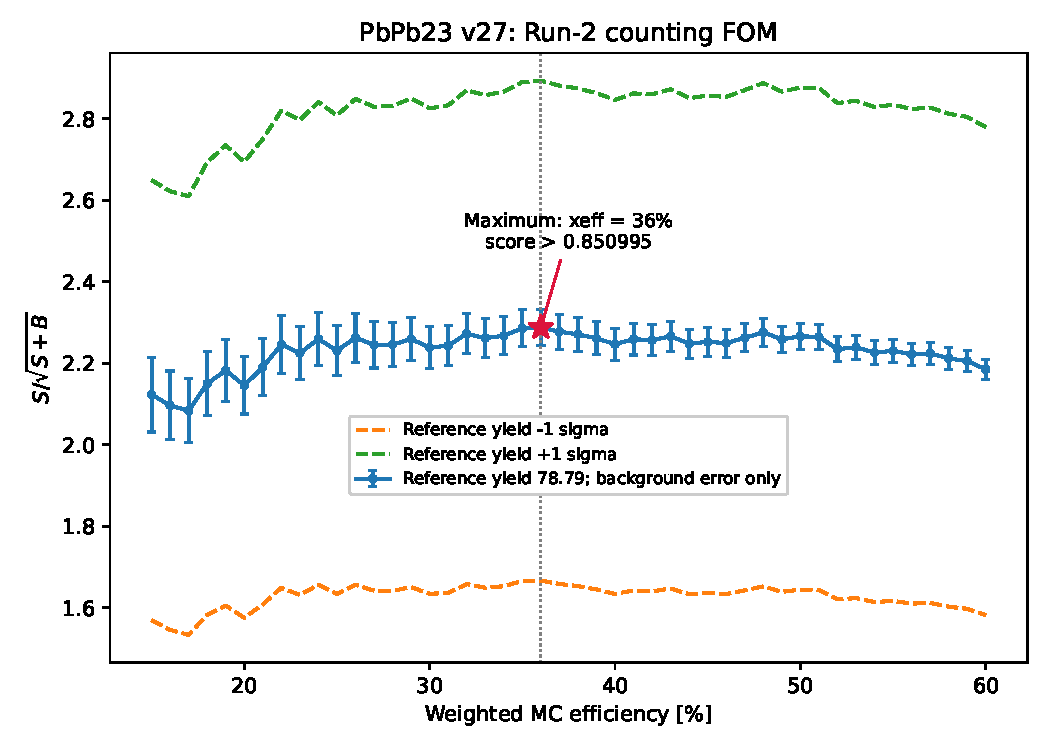
\includegraphics[width=\linewidth,height=0.46\textheight,keepaspectratio]{figures/20260916/fom/fom_xeff.pdf}
    \column{0.49\textwidth}\centering
    {\small\textbf{FOM vs score threshold}}\par
    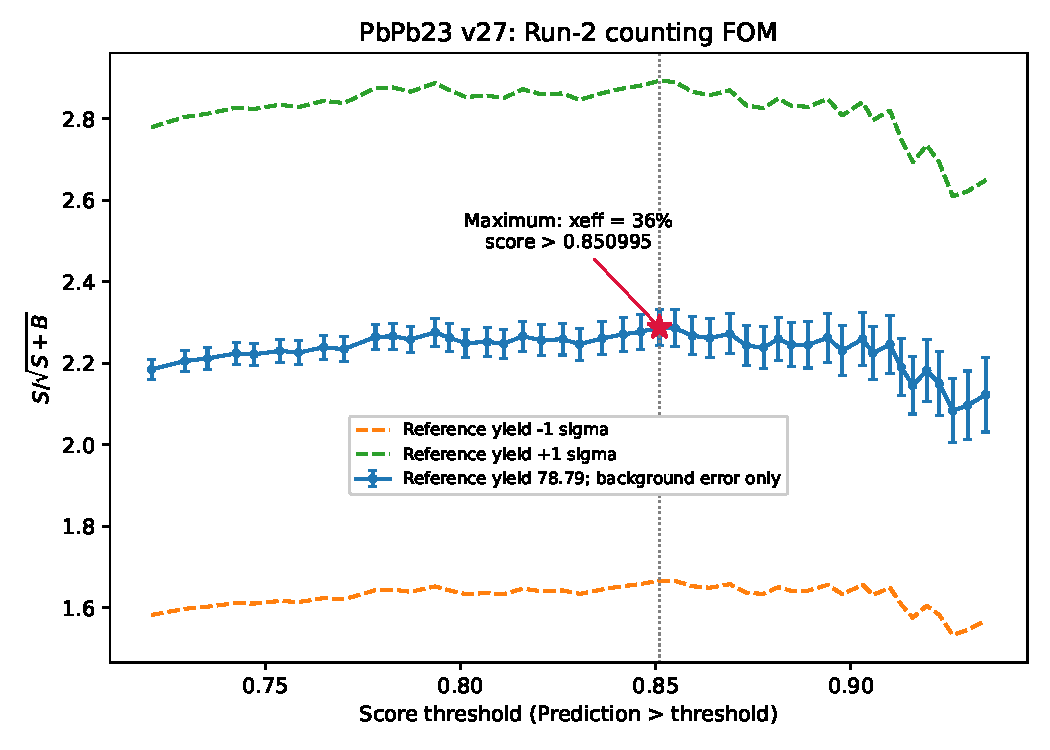
\includegraphics[width=\linewidth,height=0.46\textheight,keepaspectratio]{figures/20260916/fom/fom_score.pdf}
  \end{columns}
  {\small\textbf{Numerical maximum:} $\epsilon_X=36\%$, score $>0.850995$; $S_W=56.66$, $B_W=556.79\pm23.97$.}\par
  {\small FOM: $2.287799$ (36\%) vs $2.266093$ (50\%); improvement $0.958\%$.}\par
  {\small Broad plateau: 35\% gives $2.285971$; $N_{\rm ref}\pm1\sigma$ curves both peak at 36\%.}\par
  \vspace{0.35em}
  \caution{Error bars: background statistics only. Dashed curves: reference-yield variations, not confidence bands.}
  \caution{The 36\% point was frozen before the new DATA fit; FOM is a counting proxy, not significance.}
\end{frame}

\begin{frame}[label=p13_20260916]{Backup: configuration 5 --- fit at the FOM maximum}
  \relax
  {\small Frozen point: $\epsilon_X=36\%$, score $>0.850995$; two-peak fit over $3.62$--$4.00$ GeV.}\par
  \begin{columns}[T]
    \column{0.52\textwidth}\centering
    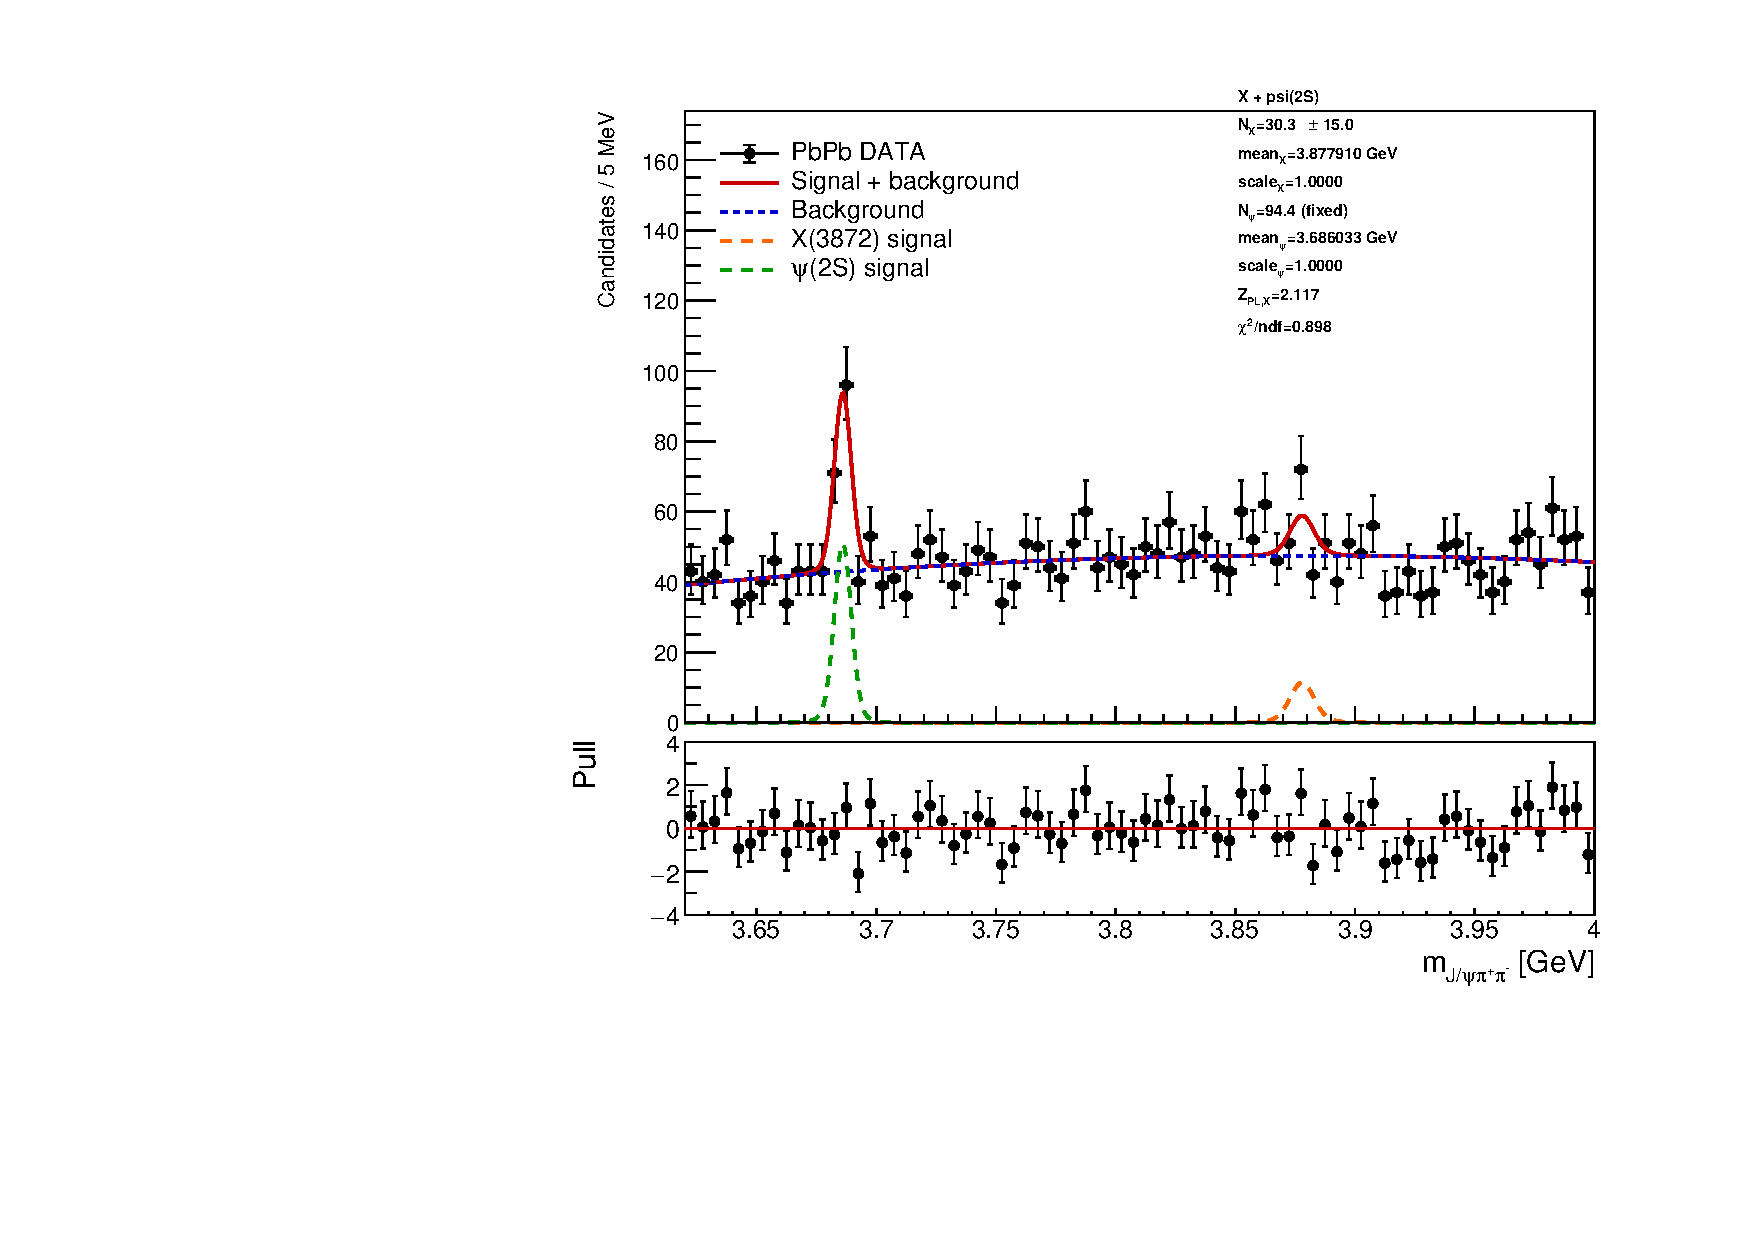
\includegraphics[width=\linewidth,height=0.54\textheight,keepaspectratio]{figures/20260916/fom/xeff36_conditional_fit.pdf}
    \column{0.45\textwidth}\small
    \textbf{36\% fit parameters}\par\vspace{0.3em}
    $\mu_X=3877.91$ MeV (fixed).\par
    $N_\psi=94.35$, $\mu_\psi=3686.03$ MeV (fixed).\par
    \vspace{0.3em}
    Means, $N_\psi$ and background shape fixed\par
    from the first fit; both MC scales fixed to 1.\par
    \vspace{0.5em}
    \begin{tabular}{@{}lcc@{}}
      \toprule
       & 36\% & 50\% reference\\
      \midrule
      FOM & 2.288 & 2.266\\
      $N_X$ & $30.33\pm15.00$ & $78.88\pm21.76$\\
      Significance & 2.117 & 3.873\\
      \bottomrule
    \end{tabular}
  \end{columns}
  \vspace{0.4em}
  {\small\textbf{Higher FOM did not increase the observed significance in this DATA sample.}}\par
  \caution{Broad FOM plateau; no final working point selected.}
\end{frame}
